% !TEX TS-program = xelatex
% !TEX encoding = UTF-8 Unicode
\documentclass[10pt,aspectratio=1610]{beamer}
%\documentclass[10pt]{beamer}

\usetheme[progressbar=frametitle]{metropolis}
\usepackage{appendixnumberbeamer}


\usepackage{booktabs}
\usepackage[scale=2]{ccicons}

\usepackage{pgfplots}
\usepgfplotslibrary{dateplot}

\usepackage{xspace}

\usepackage{bm}

% Color definitions 
%\usepackage[dvipsnames]{xcolor}

% Remove "Figure #" from figures
\setbeamertemplate{caption}{\raggedright\insertcaption\par}

% Custom commands
% Metropolis theme name 
\newcommand{\themename}{\textbf{\textsc{metropolis}}\xspace}

% Derivatives
\newcommand{\pfrac}[3][]{\frac{\partial^{#1} #2}{\partial #3^{#1}}}
\newcommand{\dd}[3][]{\frac{\mathrm{d}^{#1} #2}{\mathrm{d} #3^{#1}}}
\newcommand{\pp}[2][]{\partial^{#1}_{#2}}


\newcounter{example}
\stepcounter{example}
\newcounter{exercise}
\stepcounter{exercise}

\renewcommand{\vec}{\mathbf}
\newcommand{\varone}{\vec{x}}
\newcommand{\argone}{(t,\varone)}
\newcommand{\R}{\mathbb{R}}
\newcommand{\CC}{\mathbb{C}}
\newcommand{\Q}{\mathbb{Q}}
\newcommand{\Z}{\mathbb{Z}}
\newcommand{\N}{\mathbb{N}}
\newcommand{\norm}[1]{\left\lVert#1\right\rVert}
\newcommand{\fone}{\vec{f}}
\newcommand{\ftwo}{\vec{g}}
\newcommand{\fthr}{\vec{h}}
\newcommand{\ffor}{\bm{\phi}}
\newcommand{\opone}{\mathcal{L}}
\newcommand{\optwo}{\mathcal{G}}
\renewcommand{\Re}{\operatorname{Re}}
\newcommand{\iprod}[2]{\langle #1,#2 \rangle}
\newcommand{\diff}{\mathrm{d}}
\newcommand{\fouriert}{\mathcal{F}}

\title{Distributions and Fourier transform}
\subtitle{The infinite domain}
\date{18/3/2021}
\date{}
%\author{18.303 Linear Partial Differential Equations: Analysis and Numerics}
\institute{18.303 Linear Partial Differential Equations: Analysis and Numerics}
\titlegraphic{\hfill
\includegraphics[height=2em]{../MIT-logo.pdf}}

\begin{document}
	
	\maketitle
	
%	\begin{frame}{Table of contents}
%		\setbeamertemplate{section in toc}[sections numbered]
%		\tableofcontents%[hideallsubsections]
%	\end{frame}

\begin{frame}{Distributions}
	\begin{columns}
	\column{0.5\textwidth}
	Let's start with an example. Consider the series of functions
	\[ f_n(x) = \begin{cases}
		n(1 - |x|n), & -1/n < x < 1/n \\
		0, & \text{otherwise.}
	\end{cases} \]
	
	\onslide<2->{
	We see that $ f_n $ is not bounded by any number so it doesn't converge to an ordinary function. However,
	\[ \int_\R f_n(x) \diff x = 1 \]
	for all $ n $.} 
%	\column{0.08\linewidth}
	\column{0.5\textwidth}
%	\vspace{4em}
	\begin{figure}
		\centering
		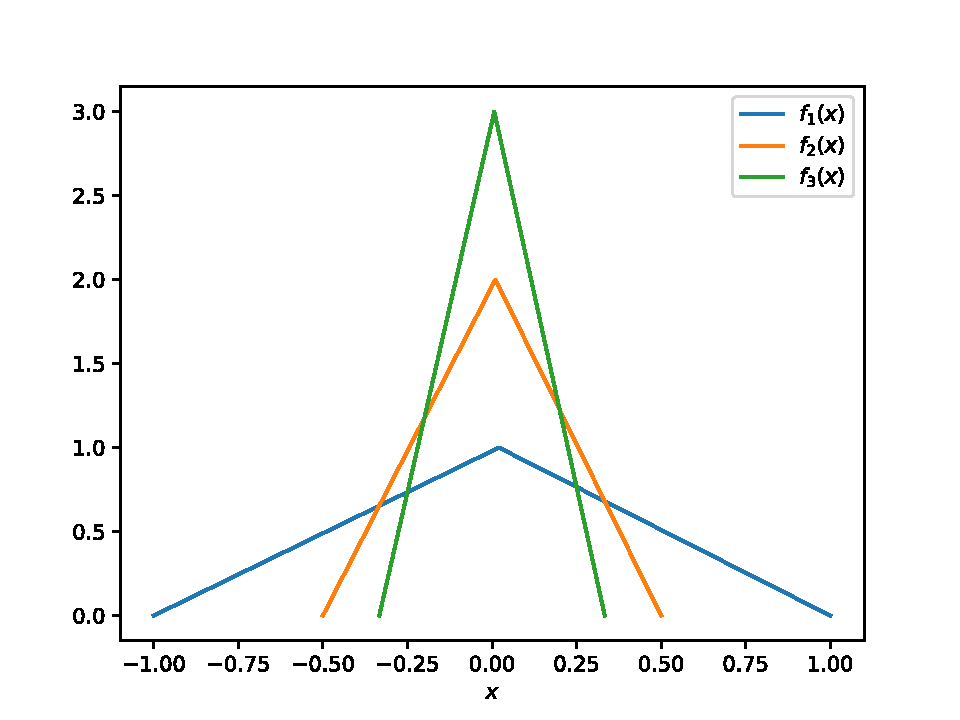
\includegraphics[width=\linewidth]{triangles.pdf}
		\caption{Few of the functions $f_n$.}
	\end{figure}
	\end{columns}
\end{frame}

\begin{frame}
	Consider some integrable function $ g: \R \to \R $. What would the inner product
	\[ \lim_{n\to\infty} \iprod{f_n}{g} = \lim_{n\to\infty} \int_\R f_n(x) g(x) \diff x \]
	give?
	
	\pause
	The integral of $ f_n $ over the real numbers is 1 and $ f_n \geq 0 $. This implies that the inner product can be seen as some sort of weighted average of $ g $.
	
	\pause
	On the other hand, the support $ f_n $ (set where $ f_n(x)\neq 0 $) is the interval $ (-1/n,1/n) $, which is getting smaller and smaller with increasing $ n $. 
	
	\pause
	It can be shown that the limit of this sequence is $ g(0) $. 
	
	\pause
	The object that we get as the limit of $ f_n $ is called a \alert{distribution}. It can be understood through inner products with ordinary functions.
\end{frame}

\begin{frame}{The delta distribution}
	In fact, the limit $ \lim_{n \to \infty} f_n =  \delta $ is a very important distribution and is called the \alert{delta distribution}. For the delta distribution we have (as we reasoned before)
	\[ \int_\R g(x) \delta(x) \diff x = g(0). \]
	
	\pause
	More generally, we can write
	\[ \int_\R g(x) \delta(x-y) \diff x = \int_\R g(x) \delta(y-x) \diff x = g(y). \]
	
	\pause
	This distribution lives in a vector space and we have
	\[ \int_\R \left( \alpha \delta(x-y) + \beta \delta (x-z)\right) g(x) \diff x =  
	\alpha \int_\R\delta(x-y) g(x) \diff x +
	\beta \int_\R \delta (x-z) g(x) \diff x = \alpha g(y) + \beta g(z).
	\]
\end{frame}

\begin{frame}
	The delta function has a scaling property
	\[ \delta(a x) = \delta(x)/|a|. \]
	
	\pause
	This can be in fact generalized to 
	\[ \delta(f(x)) = \sum_{n:f(x_n)=0} \frac{\delta(x-x_n)}{|f'(x_n)|}, \]
	where the sum goes through all the zeroes of $ f $. 
	
	\pause
	See if you can prove this by calculating 
	\[ \int_\R \delta(f(x)) g(x) \diff x. \]
\end{frame}

\begin{frame}
	The delta distribution can also be obtained as a sequence of functions that do not have a finite support. For example, for the Gaussian distribution we have
	\[ \frac{1}{\sqrt{2\pi}\sigma} e^{-\frac{(x-x')^2}{2 \sigma^2}} \xrightarrow[\sigma \to 0]{} \delta(x-x'). \]
	
	\pause
	{\color{olive}
	The sufficient condition is that the integral of $ f_n $ approaches 1 and that for any open interval $ \Omega $ not containing 0 and any $ \epsilon>0 $, there's a $ N $ s.t. for all $ n > N $, the integral 
	\[ \int_\Omega f_n(x) \diff x < \epsilon. \]}
	
	\pause
	The limiting functions don't even have to be even. We could have chosen e.g. 
	\[ f_n(x) = \begin{cases}
		2(1-n x)n, & 0 \geq x < 1/n \\
		0, & \text{otherwise}
	\end{cases} \]
	and this would still give us the delta distribution $ \delta(0). $
\end{frame}

\begin{frame}{Fourier transform}
	We define the Fourier transform for functions $ f $ as 
	\[ \fouriert[f](\xi)=\hat{f}(\xi) = \int_\R e^{-2\pi i \xi t} f(t) \diff t. \]
	
	\pause
	It has the inverse transform defined as 
	\[ \fouriert^{-1} (\hat{f})(t) = f(t) = \int_\R e^{2\pi i \xi t} \hat{f}(\xi) \diff \xi. \]
	Notice that the sign of the exponential changes here.
	
	\pause
	{\color{olive} Fourier transform exists for all functions with $ \int_\R |f(x)| \diff x < \infty $. This condition is sufficient but not necessary. Writing the sufficient condition requires a bit more math that we'll cover during this class.}
\end{frame}

\begin{frame}
	Fourier transforms can be generalized to $ \R^n $ by making $ \xi $ and $ t $ vectors and their multiplication a dot product i.e. 
	\[ f(\vx) =  \int_{\R^n} \hat{f}(\bm{\xi}) e^{2\pi i \bm{\xi} \cdot \vx } \diff \vx . \]
	
	\pause
	You might also see Fourier transforms like
	\[ \hat{f}(k) = \int_\R e^{-ikx} f(x) \diff x, \]
	that has the inverse 
	$$ f(x) = \frac{1}{2\pi} \int_\R e^{ikx} f(k) \diff k. $$
	
	\pause
	Other variants have the normalization constant in the $ \frac{1}{2\pi} $ in the transform instead of the inverse transform. There's also a unitary version with $ \frac{1}{\sqrt{2\pi}} $ normalization for both directions. 
	
	\pause
	This might seem confusing but in the end the difference between these conventions is always about multiplying the result with some $ \pi $ dependent constant.
\end{frame}

\begin{frame}
	There's an important property of the basis functions $ e^{2\pi i \xi x} $ that we will derive here. 
	Consider 
	\[ f(x) = \int_{\R} \hat{f}(\xi) e^{2\pi i \xi x} \diff \xi. \]
	
	\pause
	Replacing  $ \hat{f} $ with its definition gives 
	\[ f(x) = \int_{\R} \left( \int_\R f(x') e^{-2\pi i \xi x'} \diff x'  \right) e^{2\pi i \xi x} \diff \xi. \]
	
	\pause
	By reordering the integral we get 
	\[ f(x) = \int_\R f(x') \left( \int e^{2\pi i \xi (x-x')} \diff \xi \right) \diff x'. \]
	
	\pause
	\textbf{Question:} what does the integral in the parentheses give?
	
	\pause
	It gives us the delta function
	\[ \int e^{2\pi i \xi (x-x')} \diff \xi = \delta(x-x'). \]
	This tells us that the basis $ \{ e^{2\pi i \xi t}\}_\xi $ is orthonormal. 
\end{frame}

\begin{frame}
	Fourier transforms have other important properties. It can for example be used to calculate the derivative:
	\[ f'(x) = \dd{}{x} \int_{\R} \hat{f}(\xi) e^{2\pi i \xi x} \diff \xi = \int_\R 2\pi i \xi \hat{f}(\xi) e^{2\pi i \xi x} \diff x = \fouriert^{-1}\left[2\pi i \xi \hat{f} \right](x). \]
	
	\pause
	Notice here that if we would use the basis functions $ e^{i k x} $, we wouldn't have the deal here with the $ 2\pi $ coefficients. This is the main reason this other definition is used. 
	
	\pause
	Another property worth mentioning is \emph{Plancherel theorem}. It states that 
	\[ \int_{\R} g^*(x) f(x) \diff x = \int_{\R} \hat{g}^{*}(\xi) \hat{f}(\xi) \diff \xi, \]
	which we can also write as 
	\[ \iprod{g}{f} = \iprod{\hat{g}}{\hat{f}}. \]
	
	{\color{olive} Here we have to assume that $ \int_{\R} |g(x)|^2 \diff x $ and $ \int_{\R} |f(x)|^2 \diff x $ are finite. }
\end{frame}

\begin{frame}{Exercise 1}
	Derive Plancherel theorem using the orthonormality of the basis $ \{ e^{2\pi i \xi x} \}_\xi. $
\end{frame}

\begin{frame}{Fourier coefficients and the Fourier transform}
	Fourier coefficients are closely related to the Fourier transform.
	
	\pause
	Consider a function that is zero outside the interval $ (-L/2,L/2) $. We have the Fourier coefficients 
	\[ \hat{F}_n = \frac{1}{L} \int_{-L/2}^{L/2} f(x) e^{2\pi i x n/L} \diff x. \]
	
	\pause
	Since $ f(x) $ is zero outside this interval, we can extend the integral to the whole line. We notice then that this is just the Fourier transform of $ f $ at $ n/L $ i.e. 
	\[ \hat{F}_n = \frac{1}{L} \hat{f}\left(\frac{n}{L}\right). \]
	
	\pause
	We write the function $ f $ using the Fourier coefficients as 
	\[ f(x) = \sum_n \hat{F}_n e^{2\pi i x n/L}. \]
	
	\pause
	Substituting $ \hat{F}_n $ gives
	\[ f(x) = \sum_{n} \frac{1}{L} \hat{f}\left(\frac{n}{L}\right) e^{2\pi i x n/L}. \]
\end{frame}

\begin{frame}
	Writing $ \xi_n = n/L $ gives 
	\[ f(x) = \sum_{n\in\Z} \frac{1}{L} \hat{f}(\xi_n) e^{2\pi i \xi_n x}. \]
	
	\pause
	We notice that $ 1/L = \xi_{n+1} - \xi_{n} = \Delta \xi $. As $ L\to \infty $, this sum tends to the Riemann integral 
	\[ f(x) = \int_\R \hat{f}(\xi) e^{2\pi i \xi x} \diff \xi. \]
	
	\pause
	The connection we derived between the Fourier coefficients and the Fourier transform tells us also that we can easily approximate the Fourier transform in a discretized setting using some algorithm for calculating the Fourier coefficients.
	
	\pause
	Last time we noticed that the time domain in the wave equation was not bounded to any box. This calculation tells us that we can interpret the function $ f(t) $ in this continuous basis as a superposition of oscillating solutions where the oscillation frequency is not bounded from below.
	
	In other words, a single oscillation may take infinite amount of time. 
\end{frame}

\begin{frame}
	\centering
	\alert{No lecture next Tuesday due to a student holiday!}
\end{frame}

\end{document}
